\documentclass{sotonbeamer}
\usepackage{amsmath}
\usepackage{amssymb}
\usepackage{physics} % for math notation
\usepackage{multicol} % for multi column lists
\usepackage{algorithm2e}

\title{The effect of trapezoidal wave rise-time on power dissipation
  for magnetic hyperthermia}

\author{Oliver Laslett\inst{1} \and Michael McPhail\inst{2} \and
  Robert Woodward\inst{2} \and Hans Fangohr\inst{1} \and Ondrej
  Hovorka\inst{1}}

\institute{ \inst{1}
  Faculty of Engineering and the Environment,\\
  University of Southampton,\\Southampton, UK \and \inst{2} Department
  of Physics,\\University of Western Australia,\\Perth, Australia }

\date{14th March 2016}

\begin{document}
\maketitle

% introduction
\begin{frame}{Magnetic hyperthermia}
  A novel therapy for treating tumours
  \vspace{5mm}
  \begin{columns}
    \begin{column}{0.49\linewidth}
      \begin{itemize}
      \item Localised heating from magnetic losses
      \item Thermoablation of tissue above 45C
      \item Improves effectiveness of radiotherapy
      \end{itemize}
    \end{column}
    \begin{column}{0.49\linewidth}
      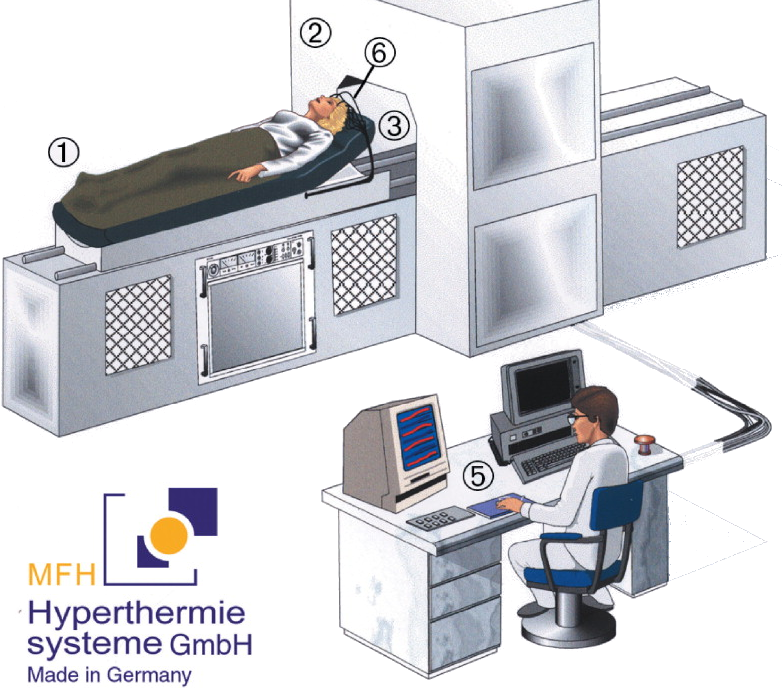
\includegraphics[width=\linewidth]{figures/hyper.png}
    \end{column}
  \end{columns}
  \footnotetext[1]{\tiny Jordan, A., et al.. J Magn Magn Mater (2001)}
\end{frame}

% optimum particle size
\begin{frame}{Required particle properties}
  \begin{columns}
    \begin{column}{0.49\linewidth}
      \begin{itemize}
      \item Magnetic properties
      \item Nontoxic and biocompatible
      \item High specific heating rates
      \item Operable at low fields
      \end{itemize}
    \end{column}
    \begin{column}{0.49\linewidth}
      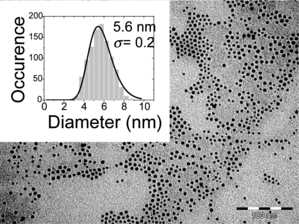
\includegraphics[width=\linewidth]{figures/particles.png}
    \end{column}
  \end{columns}
  \begin{center}
     \vspace{4mm}
     Use single domain magnetic nanoparticle iron oxides / ferrites
     \vspace{4mm}

     \textbf{Optimum particle size and applied field characteristics?}
  \end{center}
  \footnotetext[2]{\tiny Mehdaoui, B., et al.. Adv Func Mater (2011)}
\end{frame}

%% Interested in the SAR released for different particle sizes
%% we can simulate SAR by computing the MH dynamic hysteresis loop
%% This gives energy loss
\begin{frame}{Magnetic particle losses}
Obtained from hysteresis loop area (neglecting Brownian rotation):
\begin{equation*}
    \label{eq:sar_carrey}
    \textup{SPL} = fV^{-1} \int_{h_\textup{min}}^{h_\textup{max}} 2Km \textup{d}h
  \end{equation*}
  \begin{center}
    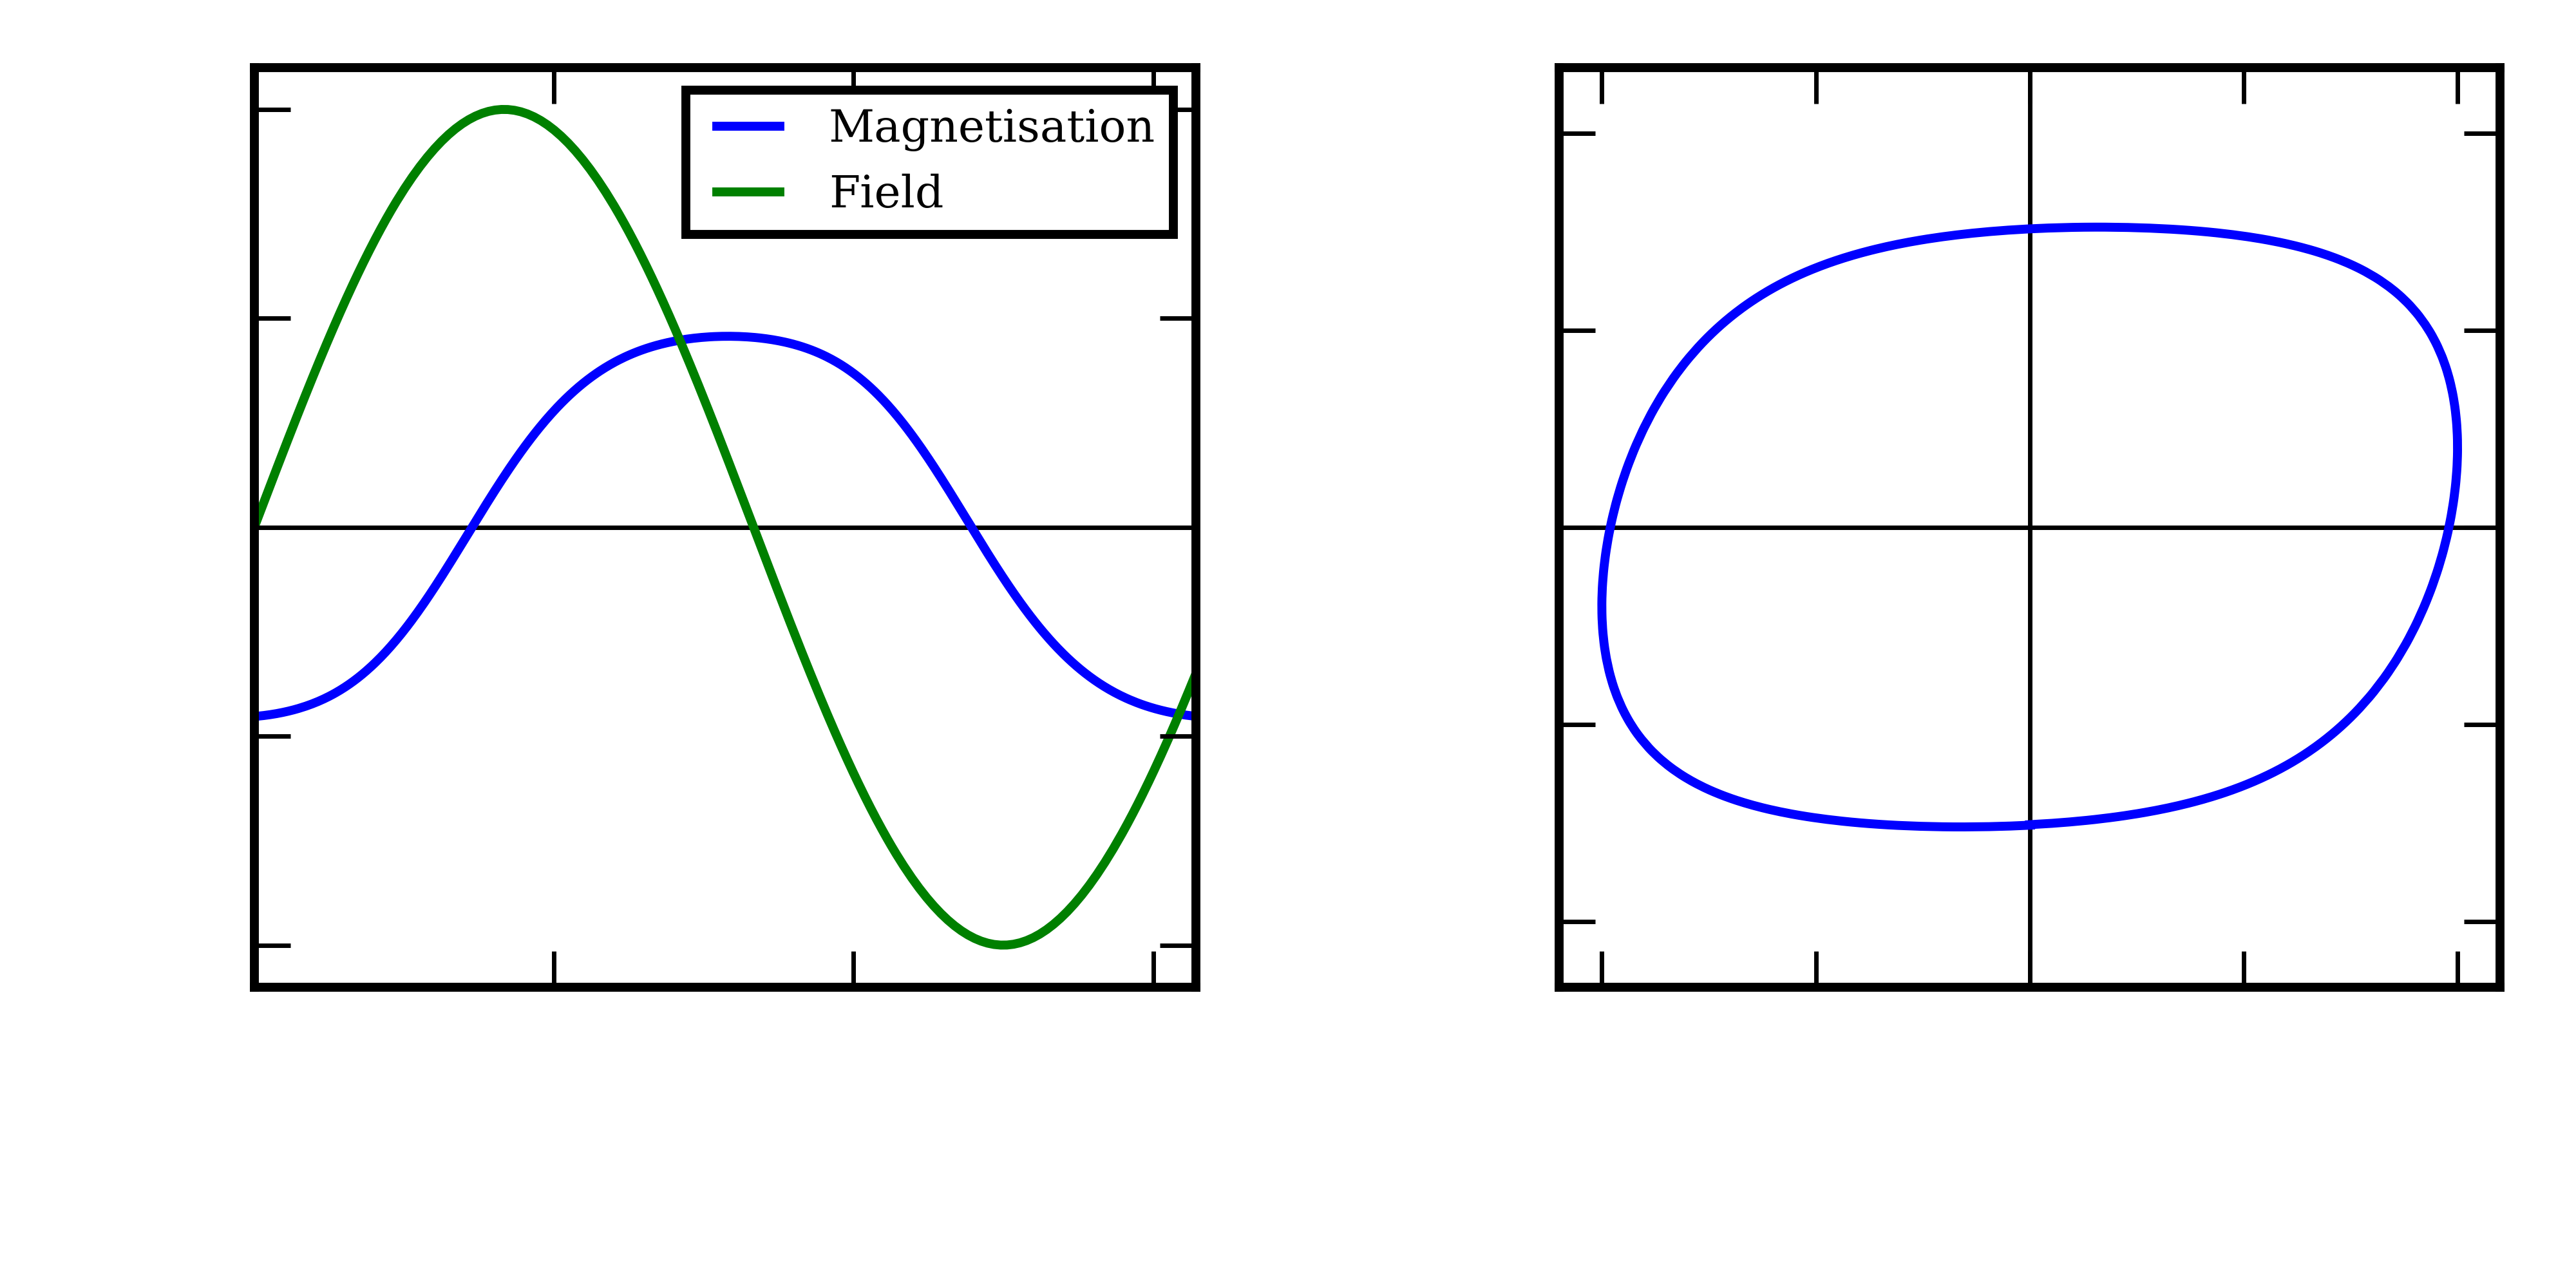
\includegraphics{figures/mt_and_mh.png}
  \end{center}
\end{frame}

%% Describe the energy barrier picture and master equation
\begin{frame}{Simulating MNP dynamics}
  Jump process limit of the LLG dynamics

  \raisebox{0.3\height}{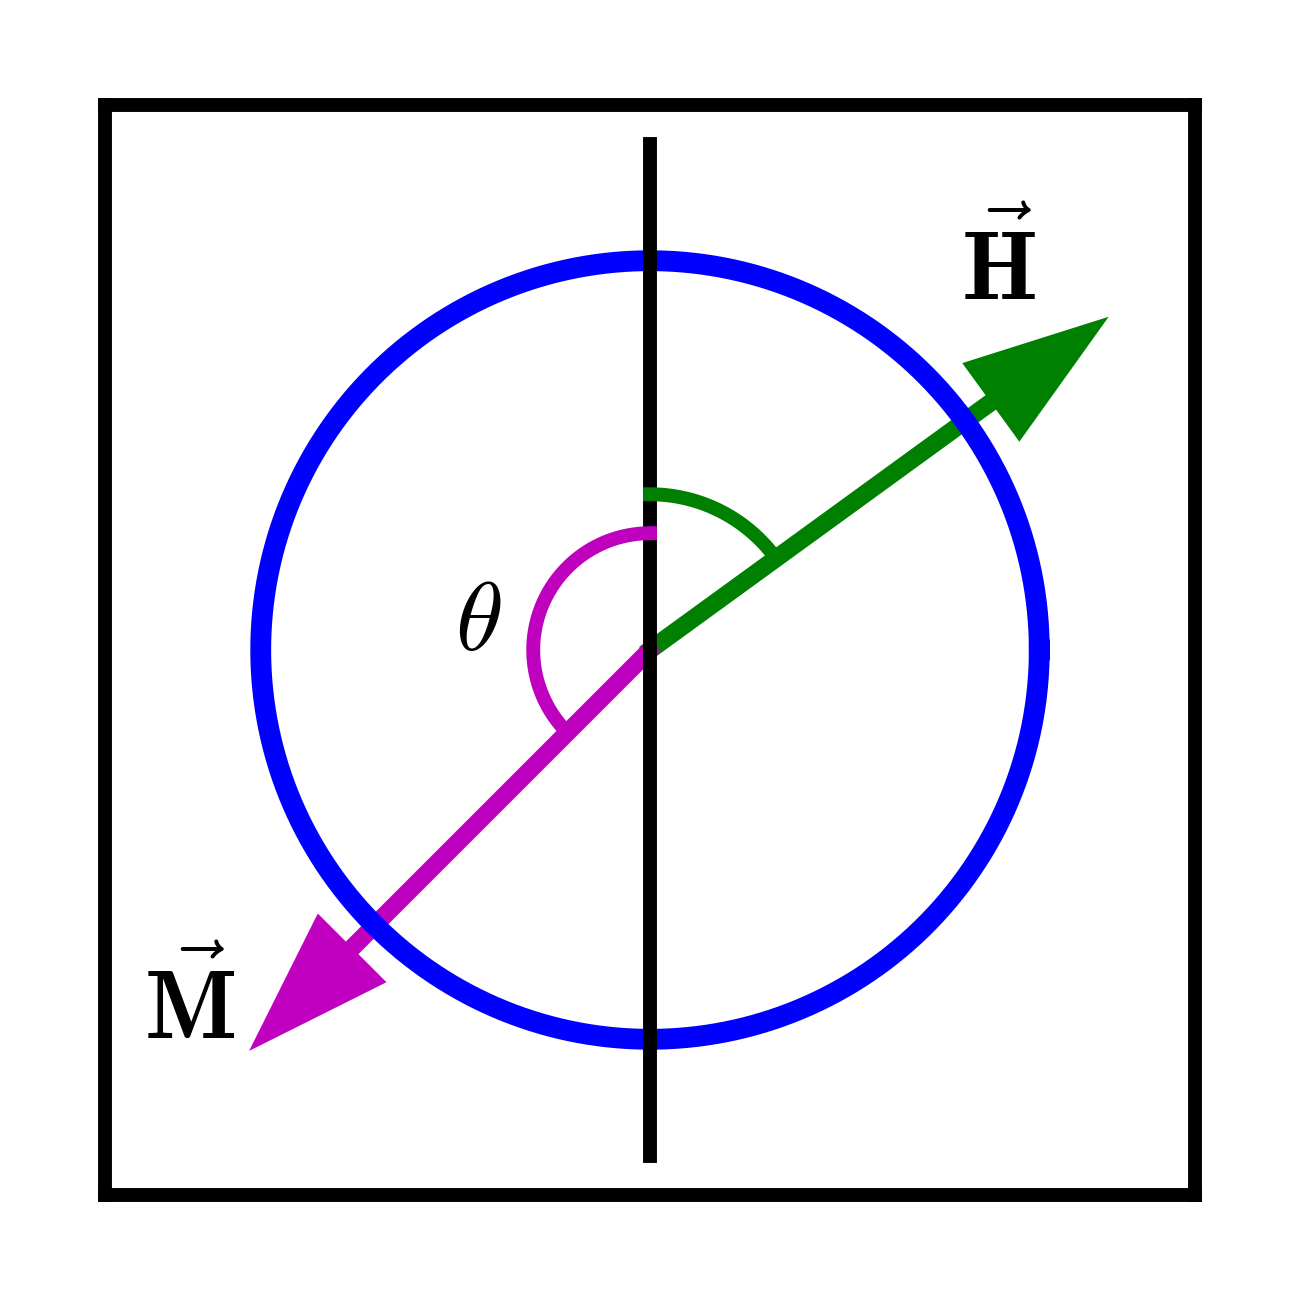
\includegraphics{figures/mnp.png}}
  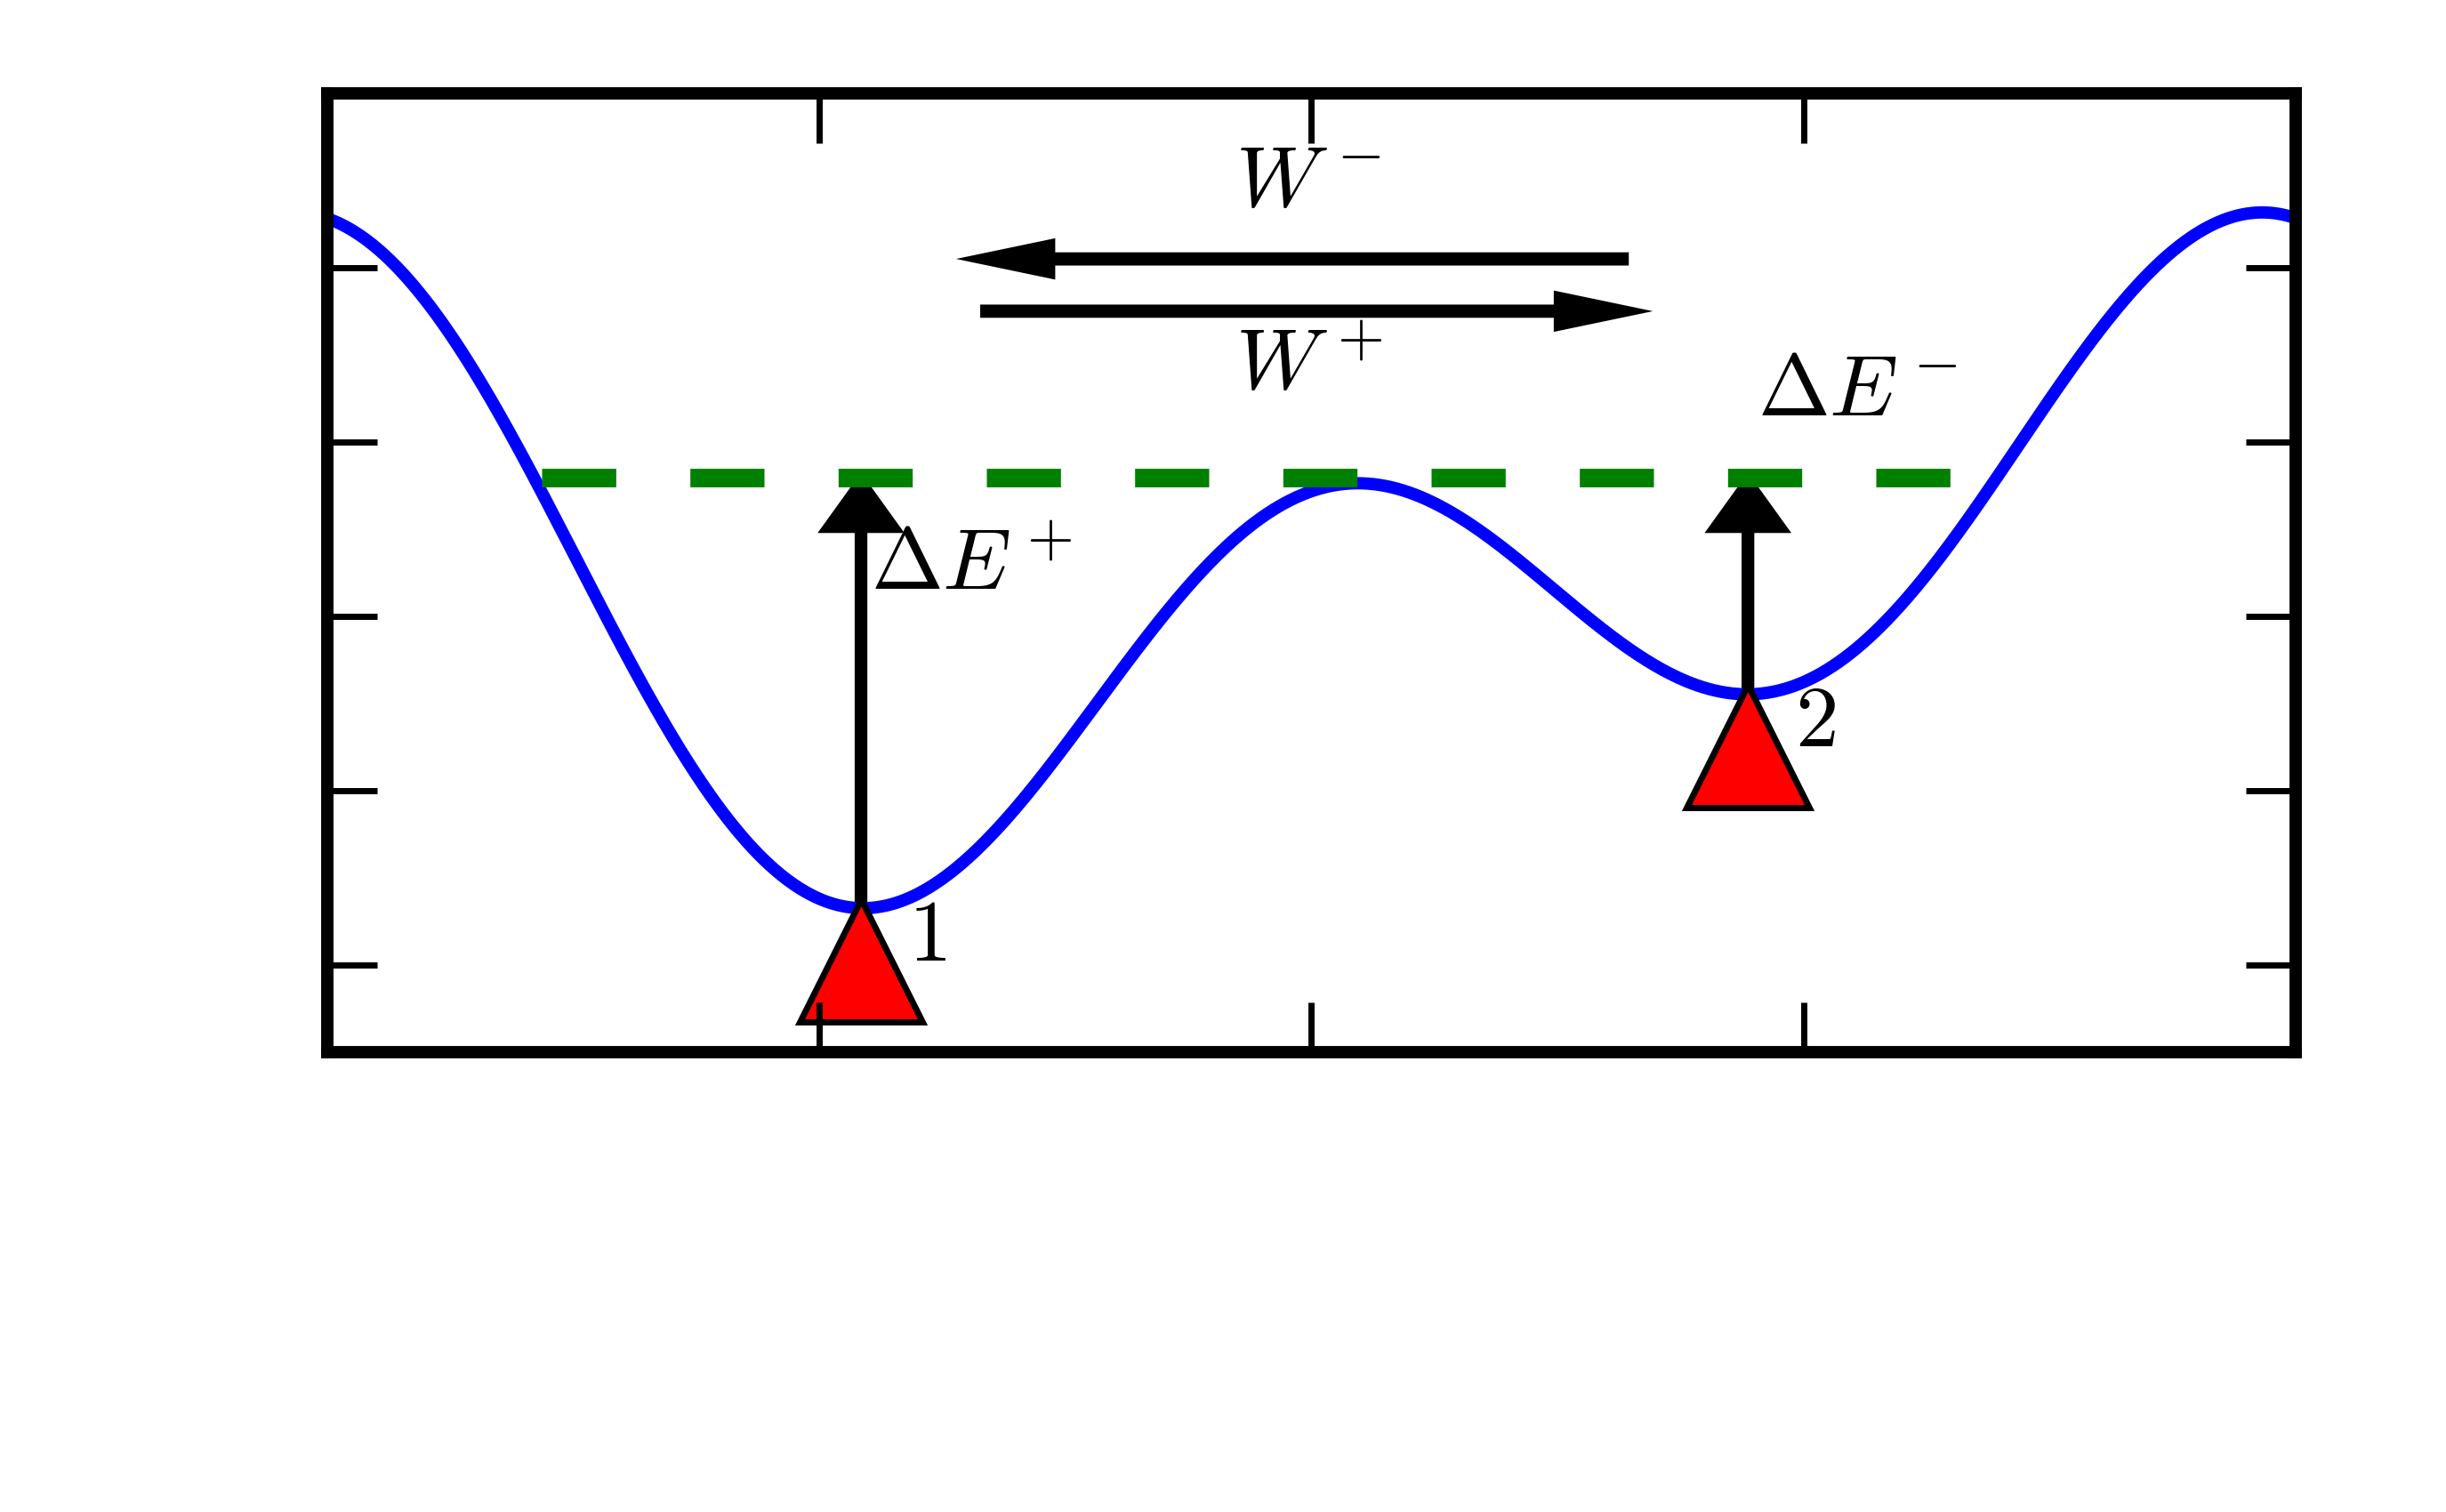
\includegraphics[scale=0.98]{figures/transitions.png}
  \vspace{-8mm}
  \center Stoner-Wohlfarth model and master equation
  \begin{align*}
    E = E_{\textup{SF}}\left( \theta, \va{H}(t)\right) \qquad
        &\dv{t} \va{p}(t) = W(t)\va{p}(t) \\
    W^\pm(t) = f_0e^{-\Delta E^\pm(t)/k_BT} \qquad
    & M(t) = p_1(t)M_1 + p_2(t)M_2
  \end{align*}
  \footnotetext[3]{\tiny Carrey, J., et.al.. J. App. Phys. (2011)}
\end{frame}

%% Psuedo code for the simulation procedure for computing the MH
%% curve
\begin{frame}{Simulating the MH curve}
  \begin{algorithm}[H]
    \KwData{Particle properties, temperature, external field}
    \KwResult{Time dependent magnetisation}
    \BlankLine
    \While{solution is not periodic $M(t_0) \neq M(t_N)$}{
      $\va{p}(t_0) \leftarrow \va{p}(t_N)$\;
    \For{$t_n$ in one field cycle}{
    Compute $H(t_n)$\;
  Compute $W_\pm(H(t_n))$\;
  Compute $\dd \va{p} /\dd t$ at $t_n$\;
  Compute $\va{p}(t_n)$ with RK4\;
  Compute $M(t_n)$\;}
Store $\va{p}(t_N)$\;
}
  \end{algorithm}
\end{frame}

%% Interested in the SAR released for different particle sizes
%% we can simulate SAR by computing the MH dynamic hysteresis loop
%% This gives energy loss
\begin{frame}{Square waveforms lead to degeneracy}
  \begin{equation*}
    \label{eq:sar_carrey}
    \textup{SPL} = fV^{-1} \int_{h_\textup{min}}^{h_\textup{max}} 2Km \textup{d}h
  \end{equation*}
  \begin{center}
    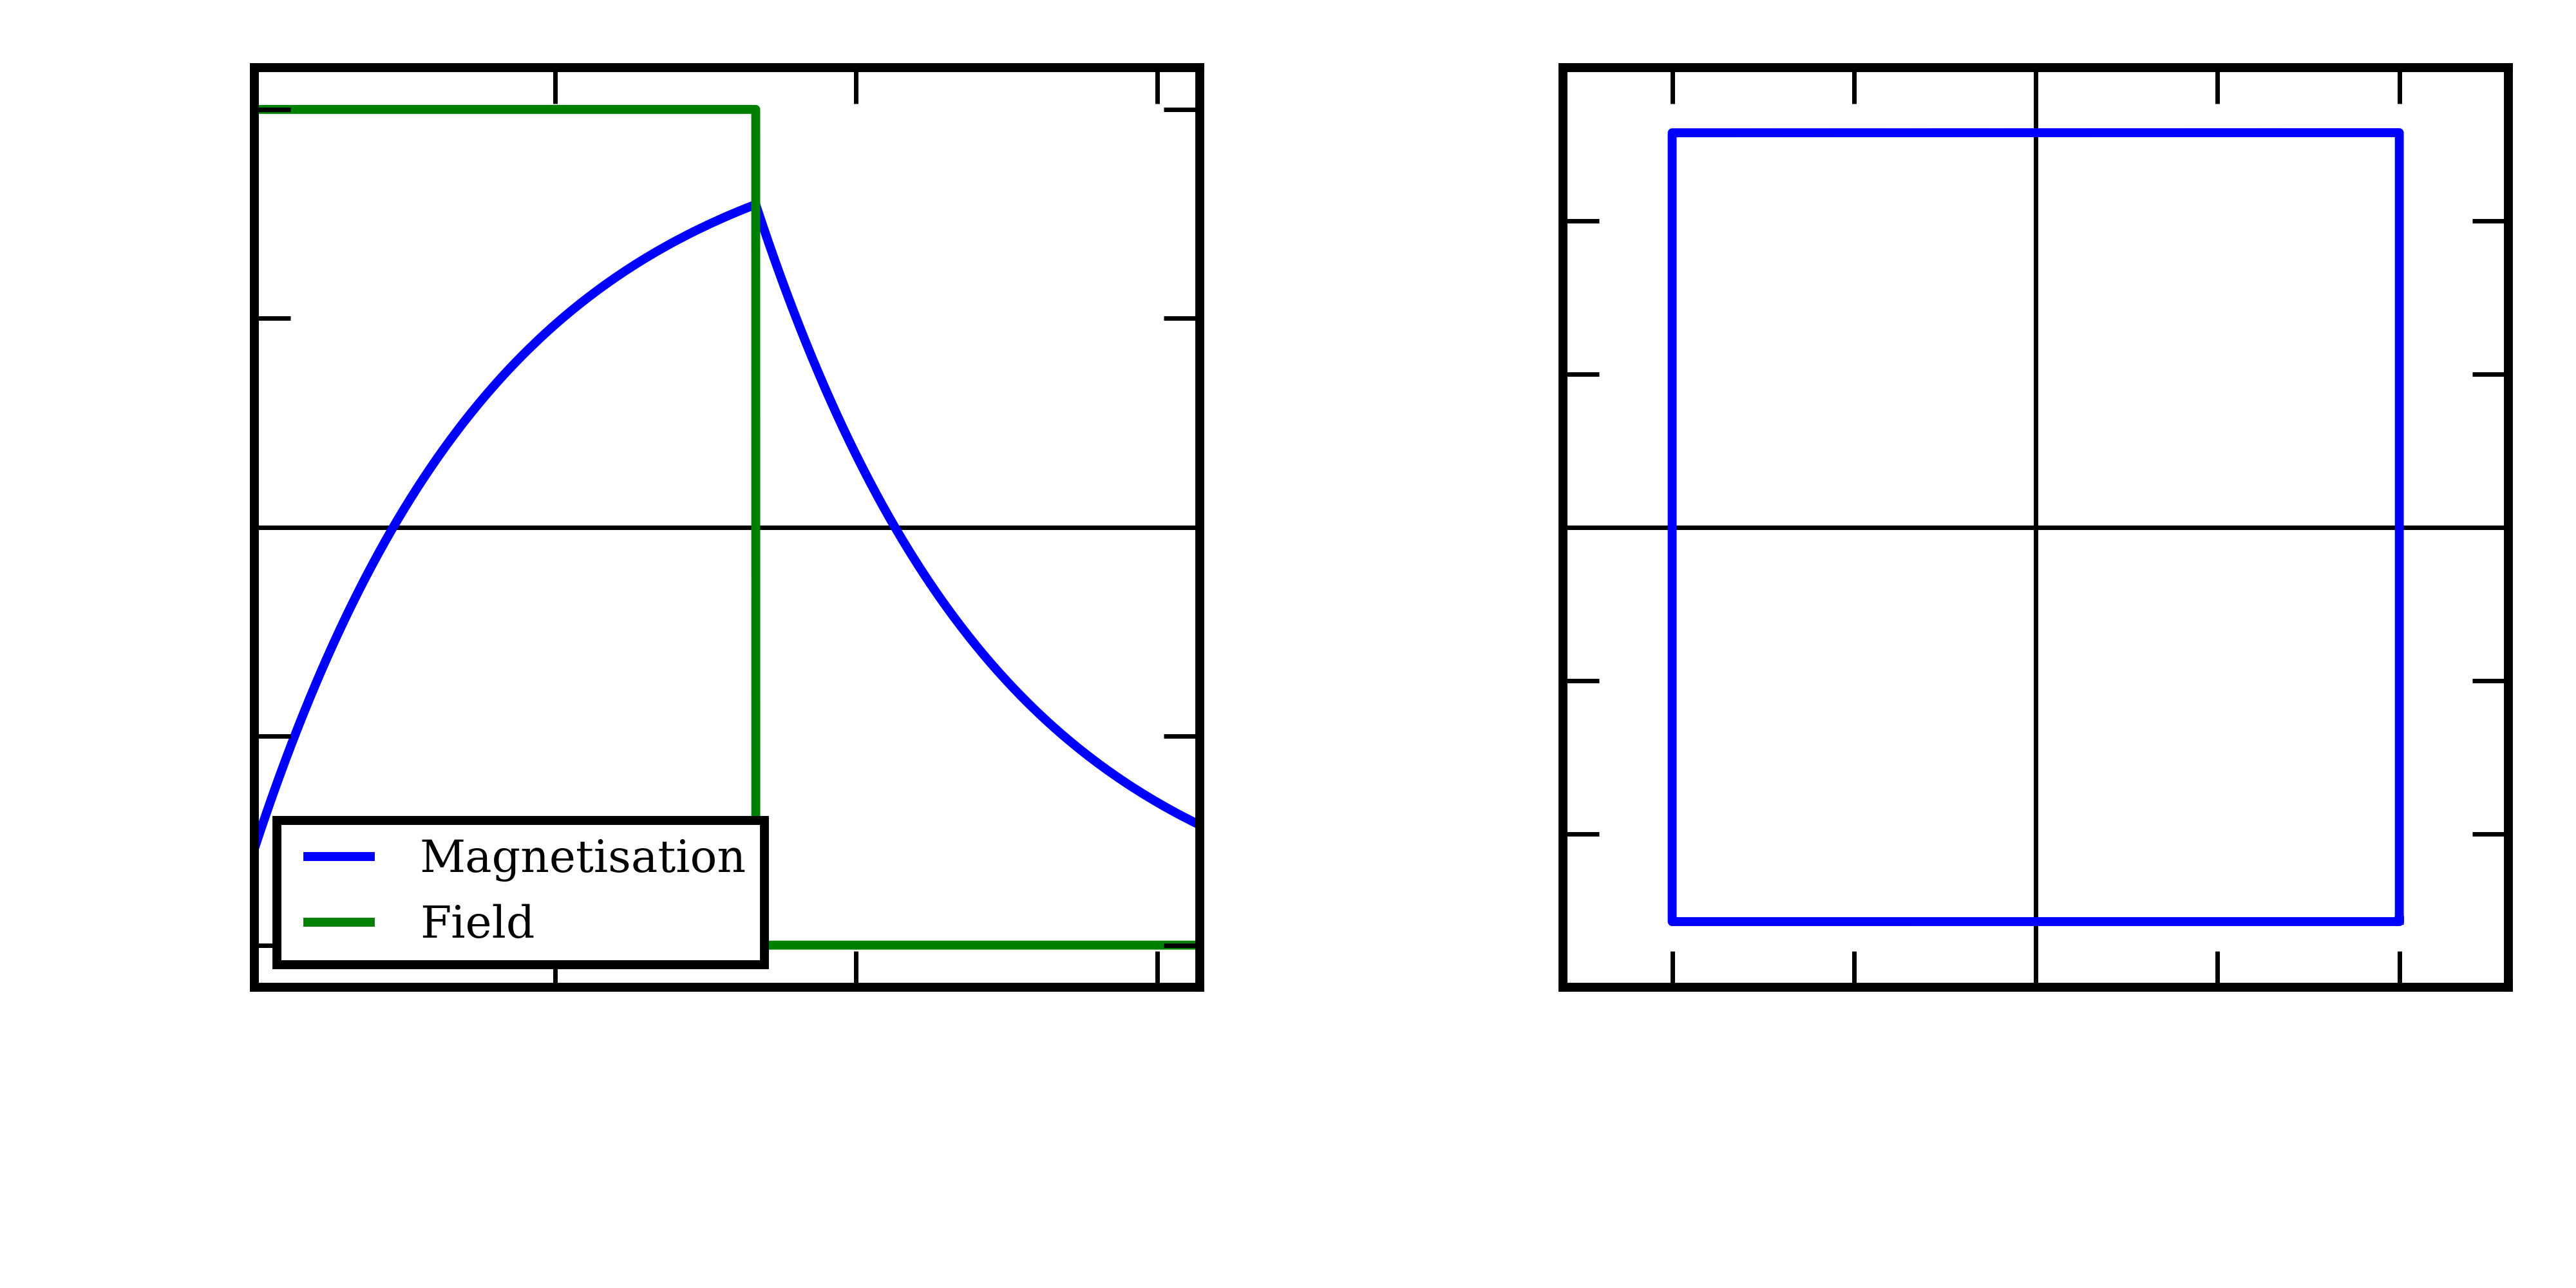
\includegraphics{figures/mt_and_mh_square.png}
  \end{center}
\end{frame}

\begin{frame}{An alternative calculation of SPL}
  Applies to arbitrary applied field waveforms
  \begin{equation*}
    \label{eq:integral}
    \textup{SPL} = fV^{-1} \int_0^T \left[ E^+(t) - E^-(
      t) \right] \dv{p_1(t)}{t} \dd t
  \end{equation*}
  \begin{itemize}
  \item Integral can be solved numerically
  \item Closed form solution for square waveform
  \item \textbf{No explicit dependence on $H$}
  \end{itemize}
  \begin{center}
    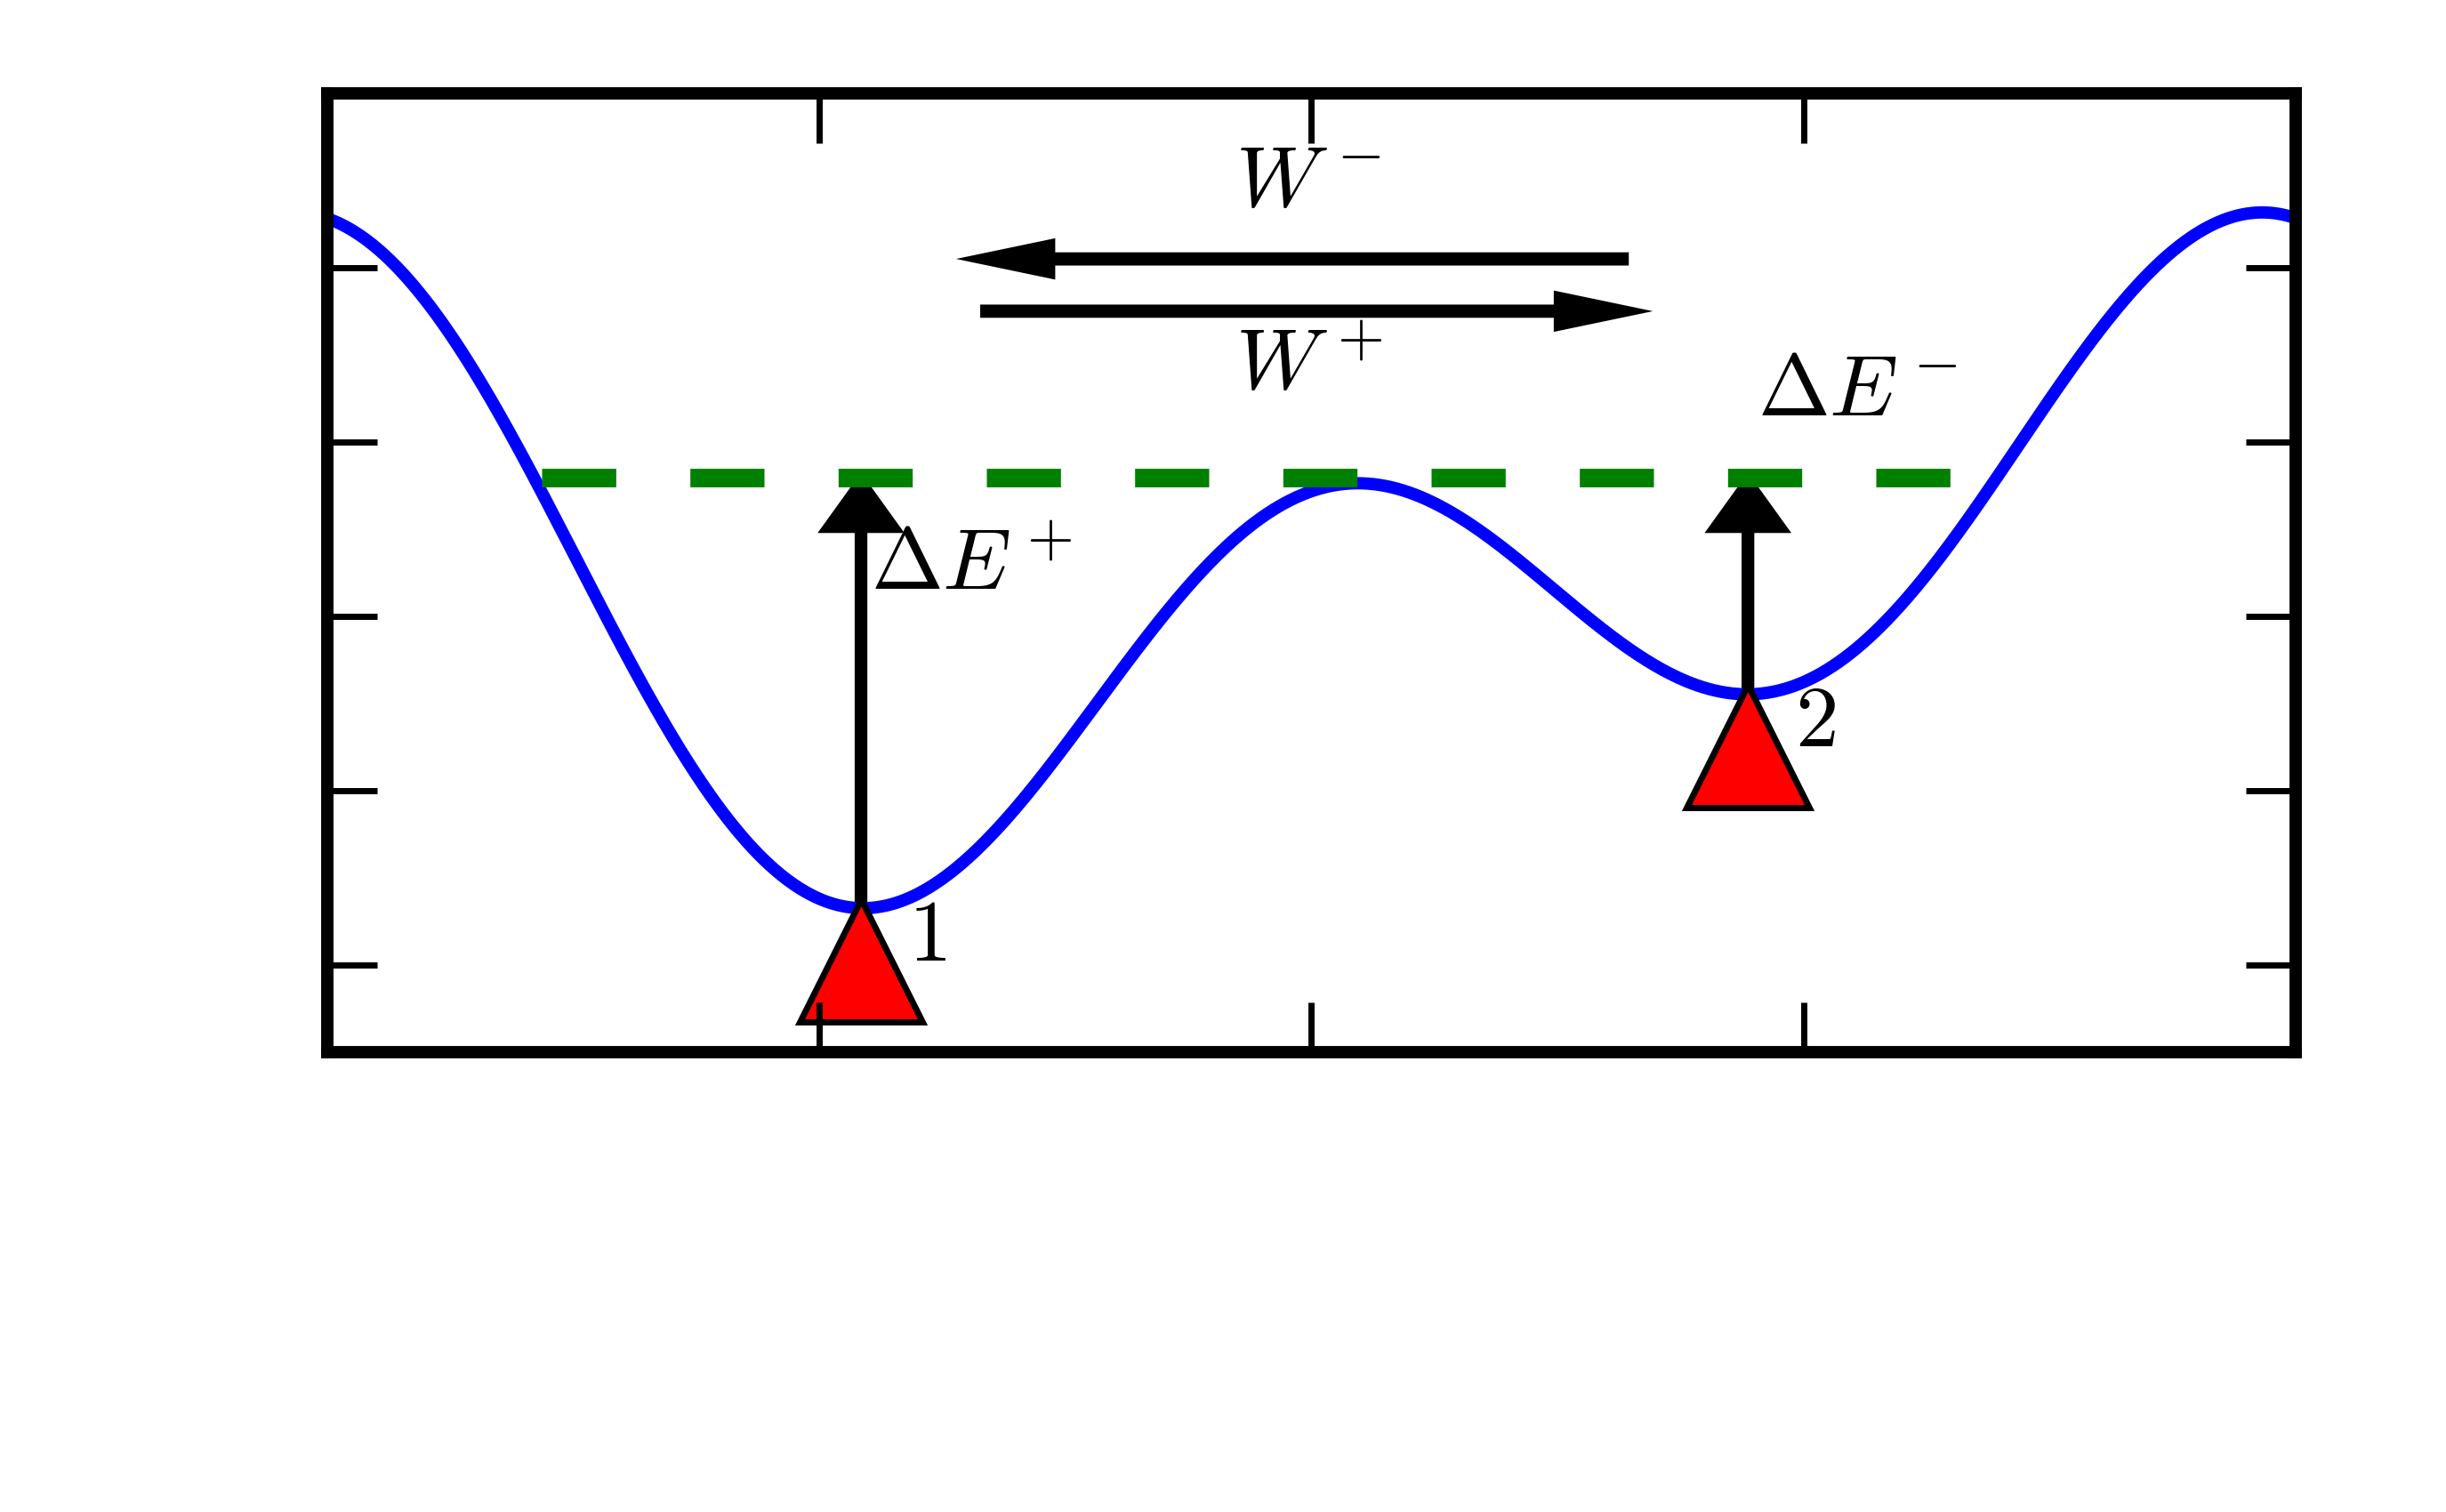
\includegraphics[width=0.4\linewidth]{figures/transitions.png}
  \end{center}
  \footnotetext[4]{\tiny McPhail, M., et.al.. \emph{In review} (2016)}
\end{frame}

\begin{frame}{An alternative calculation of SPL}
  Applies to arbitrary applied field waveforms
  \begin{equation*}
    \label{eq:integral}
    \textup{SPL} = fV^{-1} \int_0^T \left[ E^+(t) - E^-(
      t) \right] \dv{p_1(t)}{t} \dd t
  \end{equation*}
  \begin{itemize}
  \item Integral can be solved numerically
  \item Closed form solution for square waveform
  \item \textbf{No explicit dependence on $H$}
  \end{itemize}
  \begin{block}{Conditions for validity}
    \begin{multicols}{2}
      \begin{itemize}
      \item Steady-state periodic
      \item $H<H_c$
      \item Time reversal symmetry
      \item Master equation applies
      \end{itemize}
    \end{multicols}
  \end{block}
  \footnotetext[4]{\tiny McPhail, M., et.al.. \emph{In review} (2016)}
\end{frame}

\begin{frame}{Results for a single (aligned) particle}
Square wave harmonics target smaller particles
  \begin{center}
    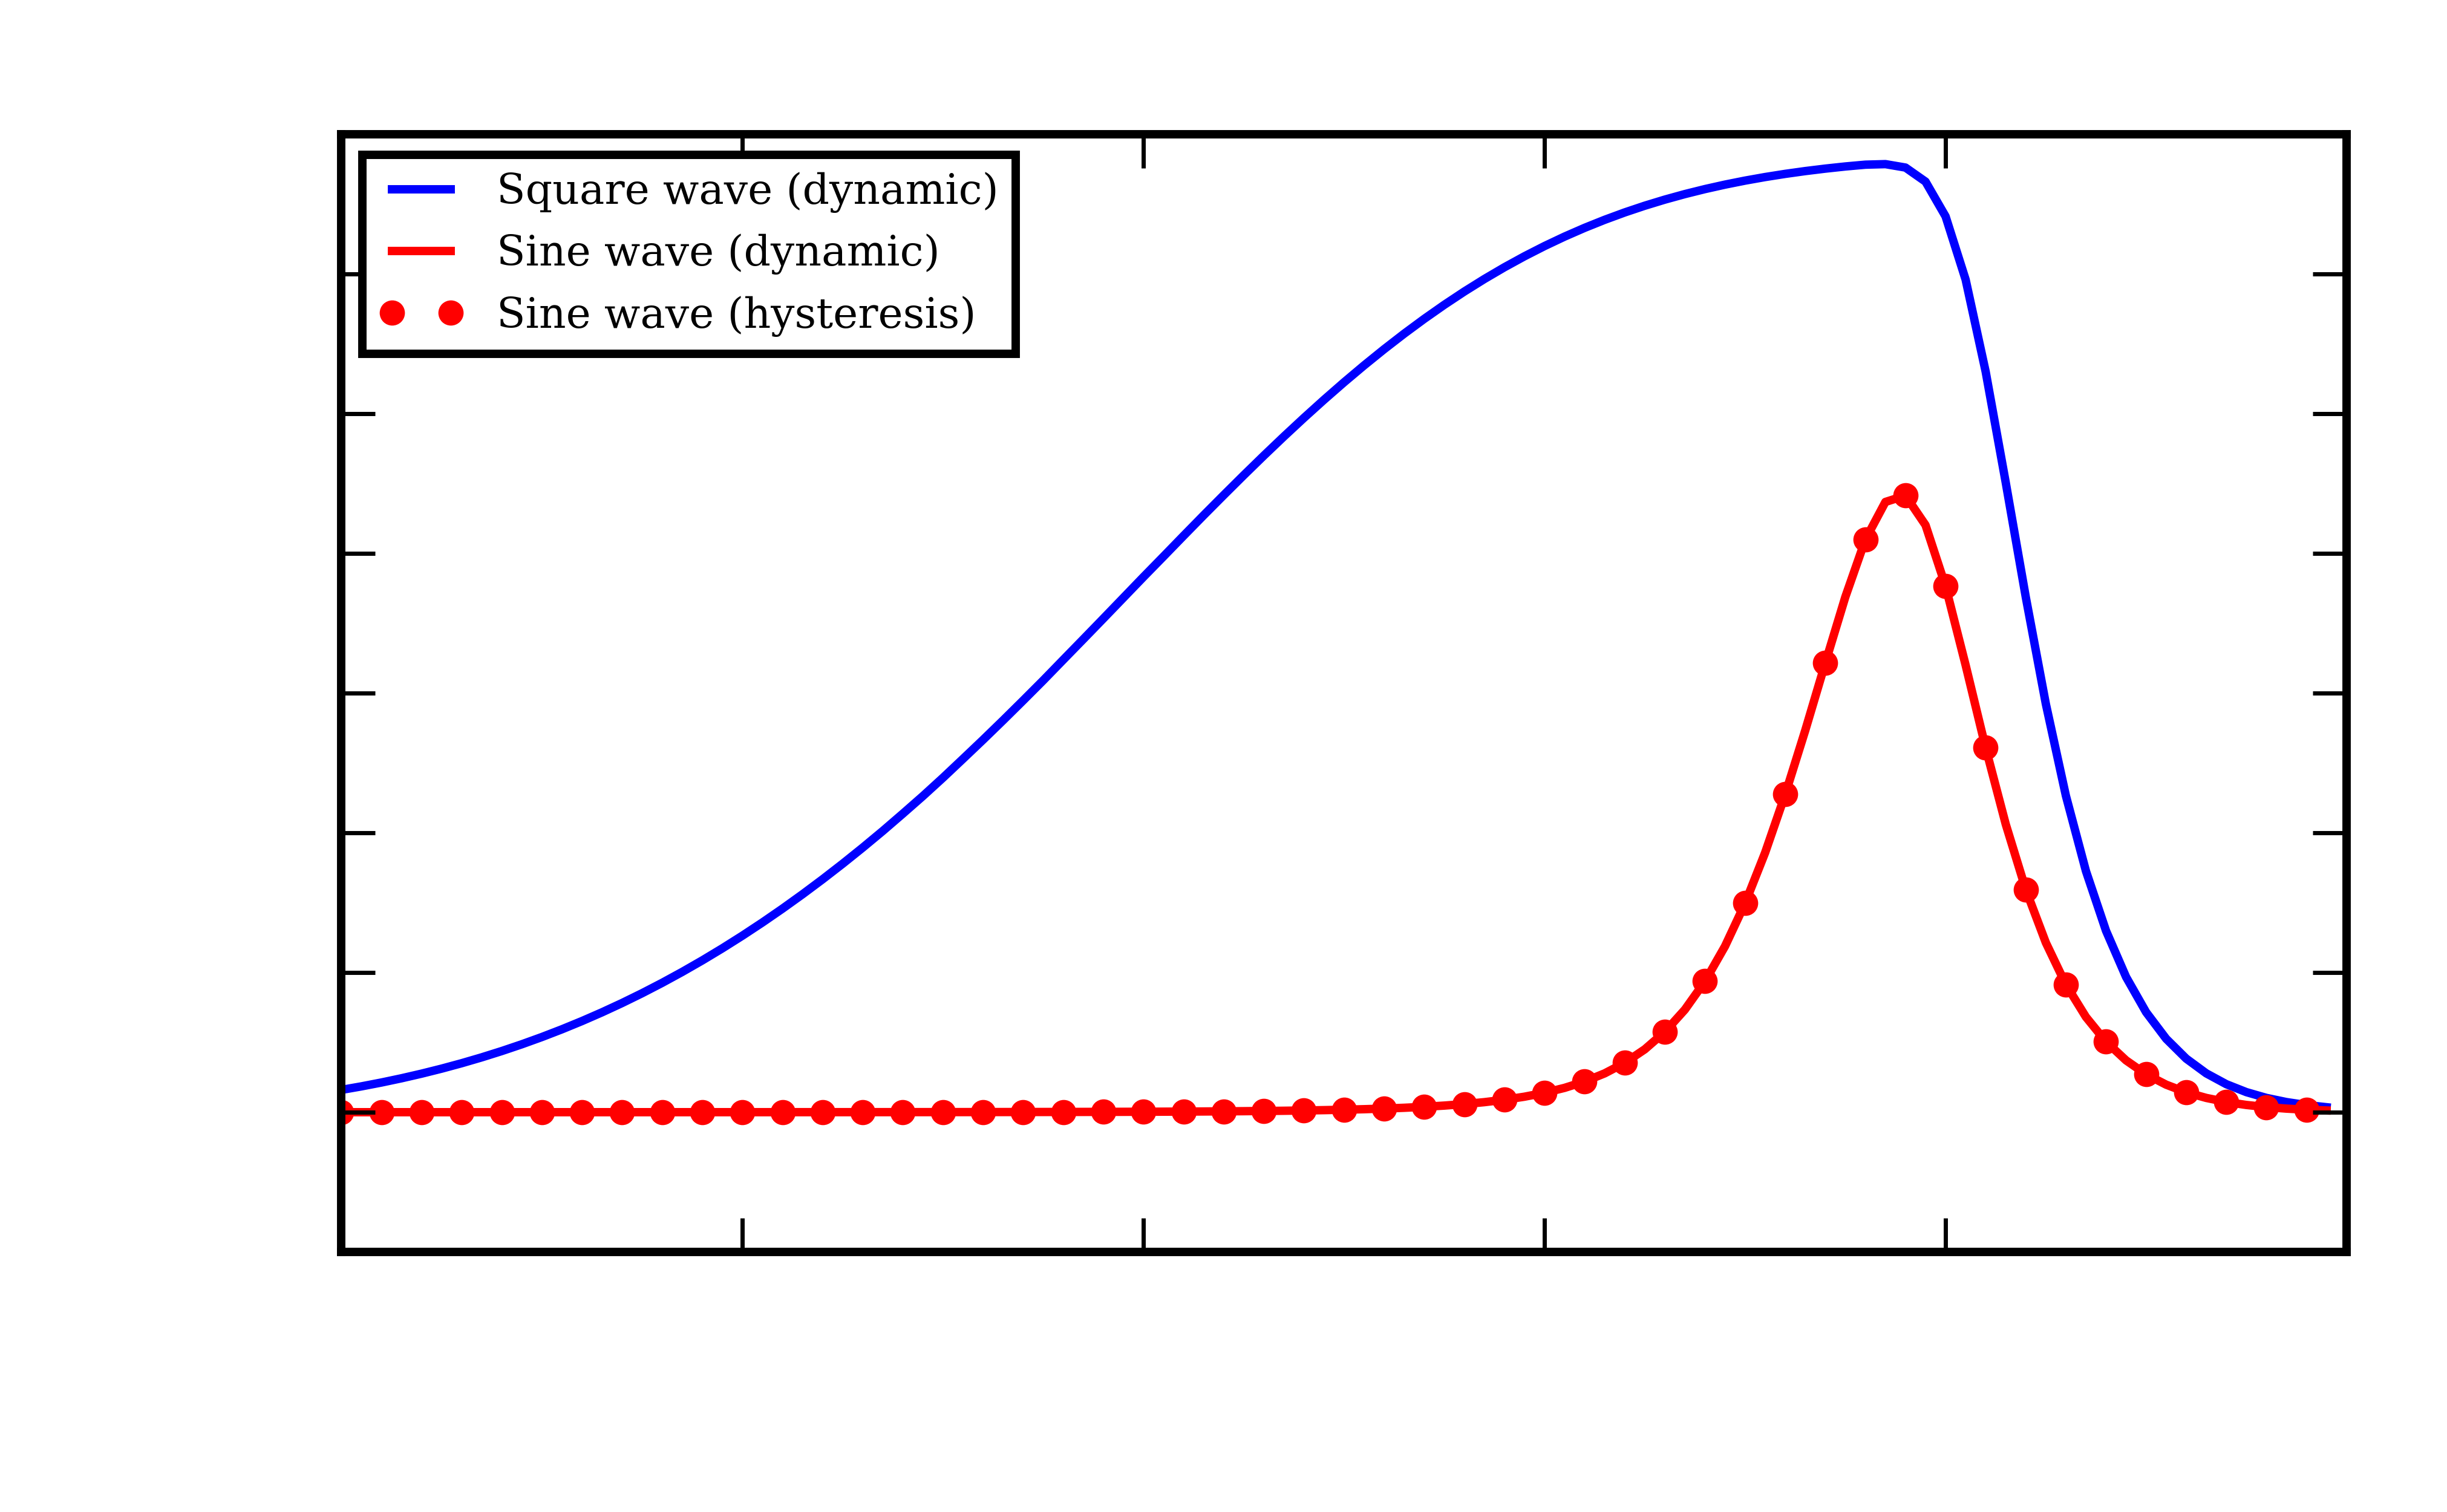
\includegraphics{figures/sineVsquare.png}
  \end{center}
\vspace{-3mm}
  {\tiny $T=298$K, $K=11k$kJ/m$^3$, $h=0.13$, $f=300$kHz}
\end{frame}

\begin{frame}{Applied trapezoidal waveform}
Harmonics quickly diminish
  \begin{center}
    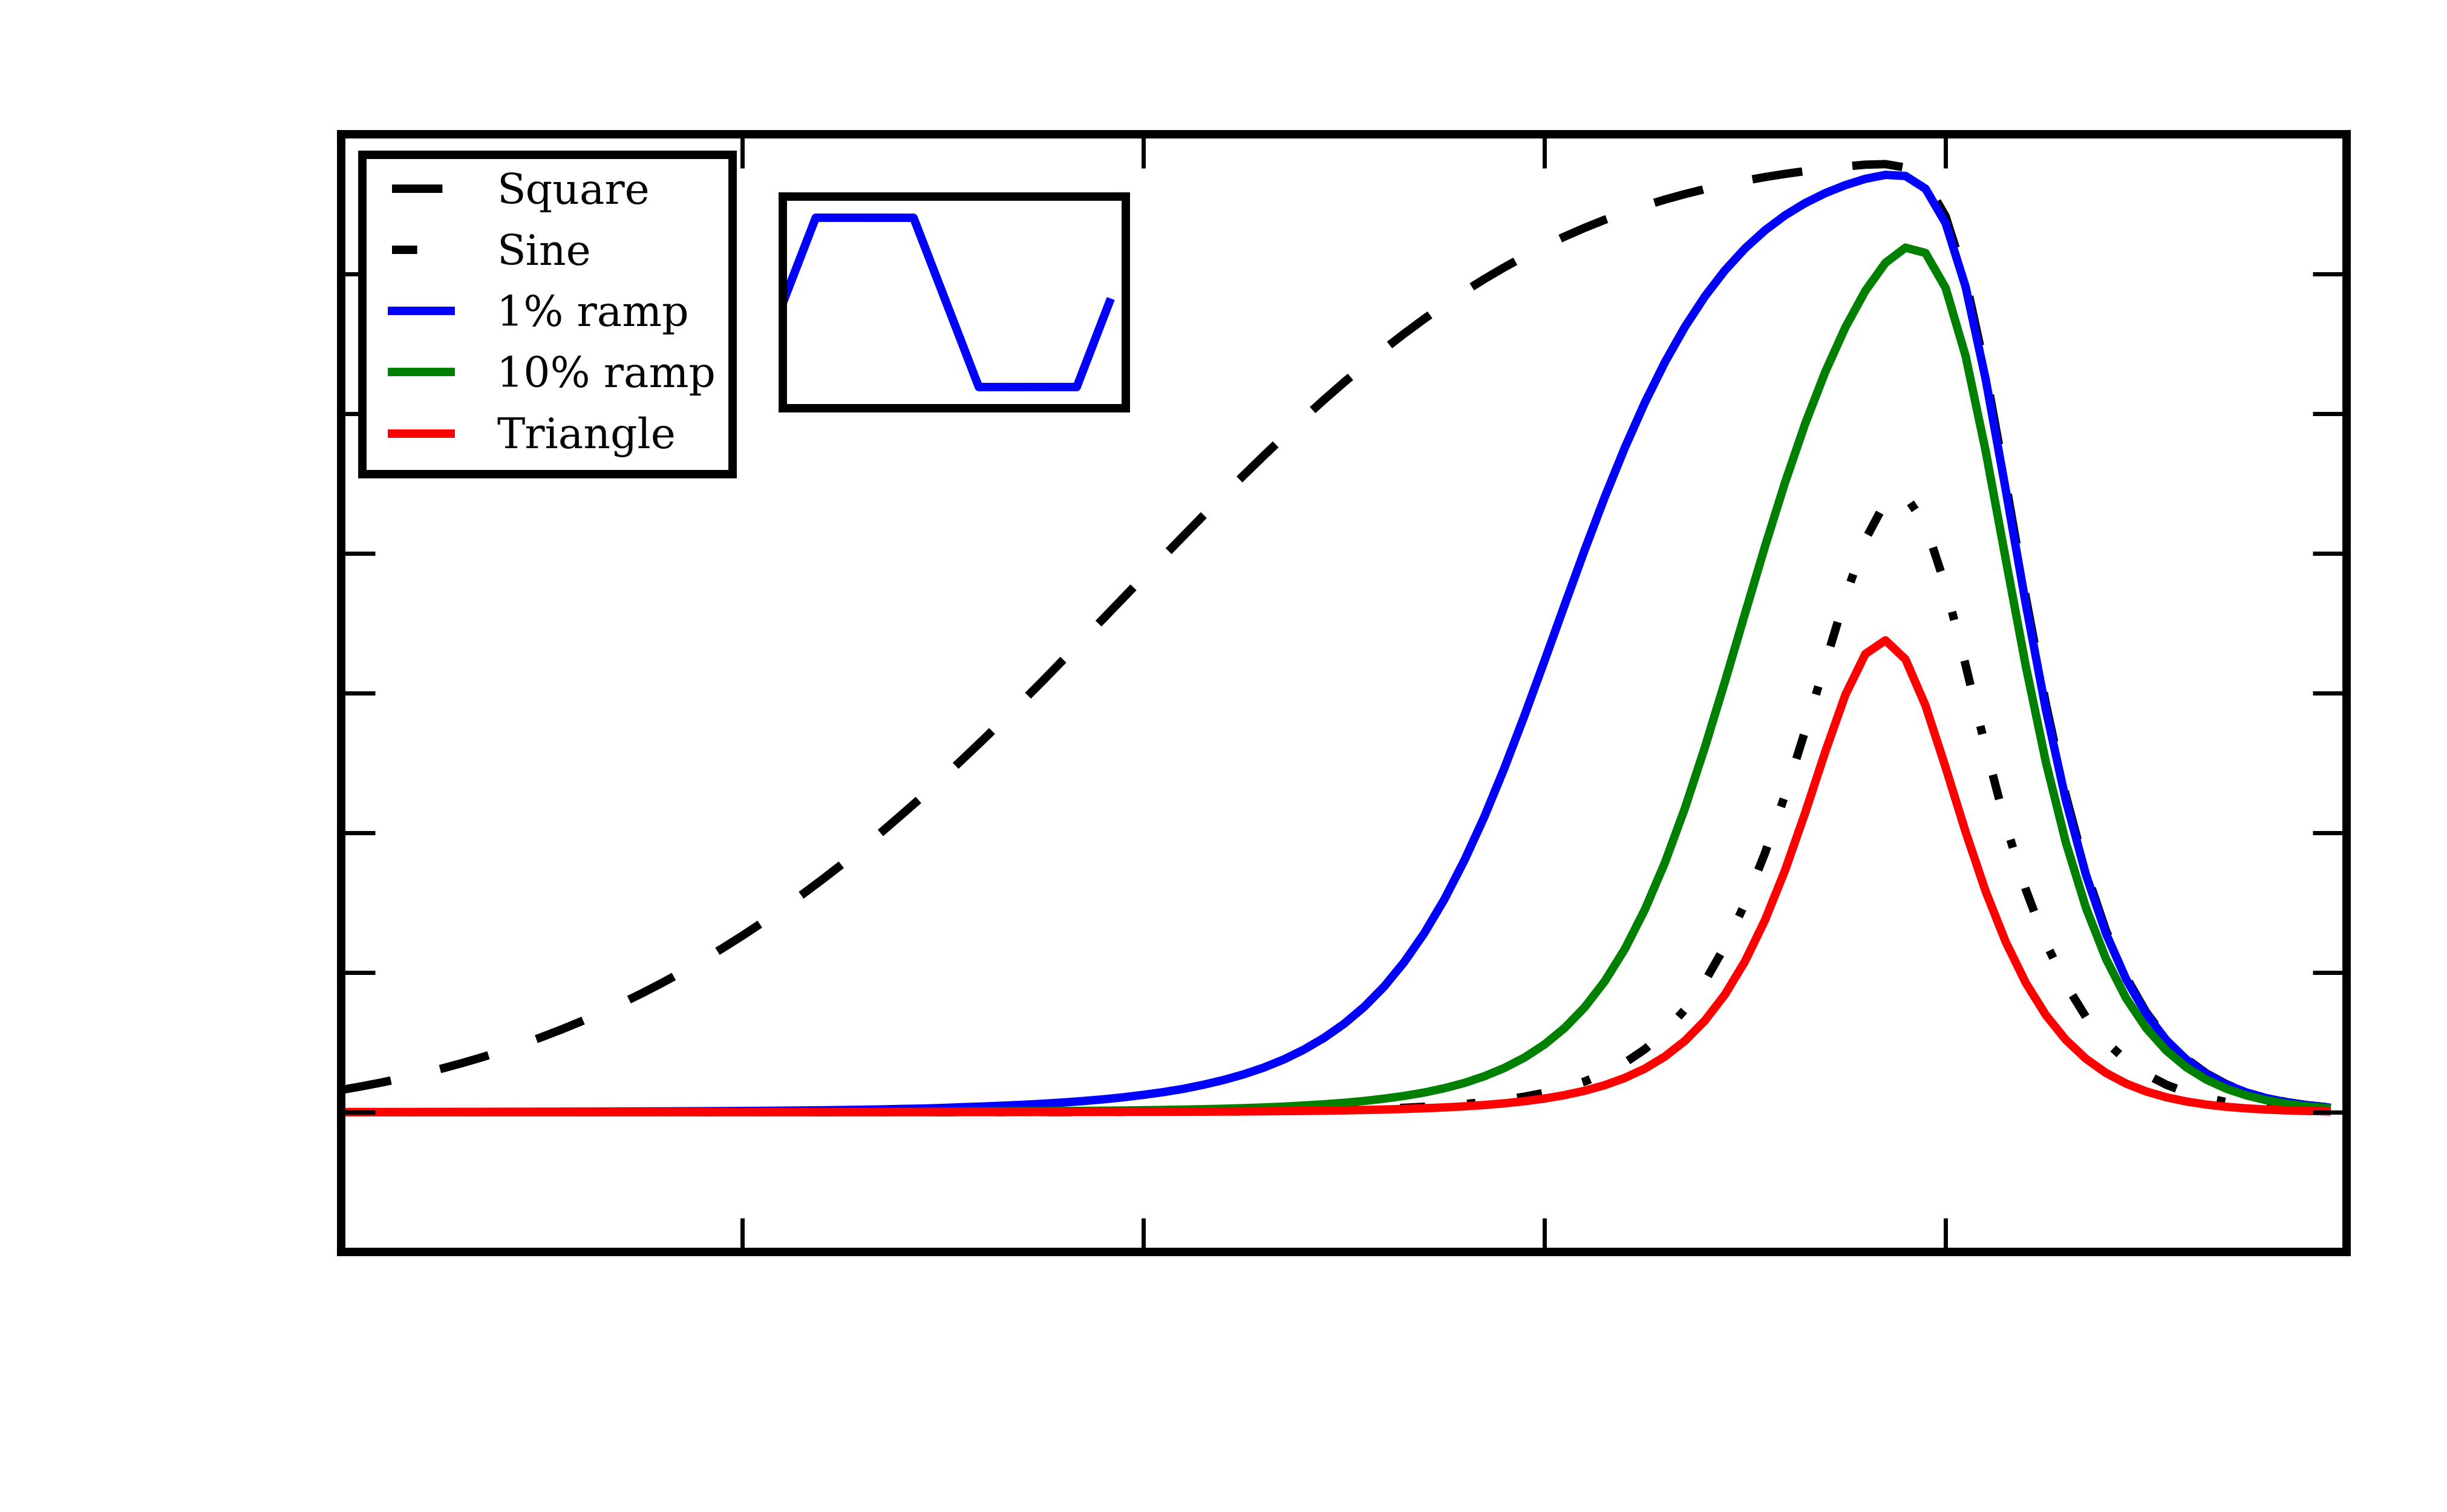
\includegraphics{figures/trap.png}
  \end{center}
\vspace{-3mm}
{\tiny $T=298$K, $K=11$kJ/m$^3$, $h=0.13$, $f=300$kHz}
\end{frame}

\begin{frame}{A realistic particle ensemble}
Lognormal size and uniform anisotropy axis distributions
  \begin{center}
    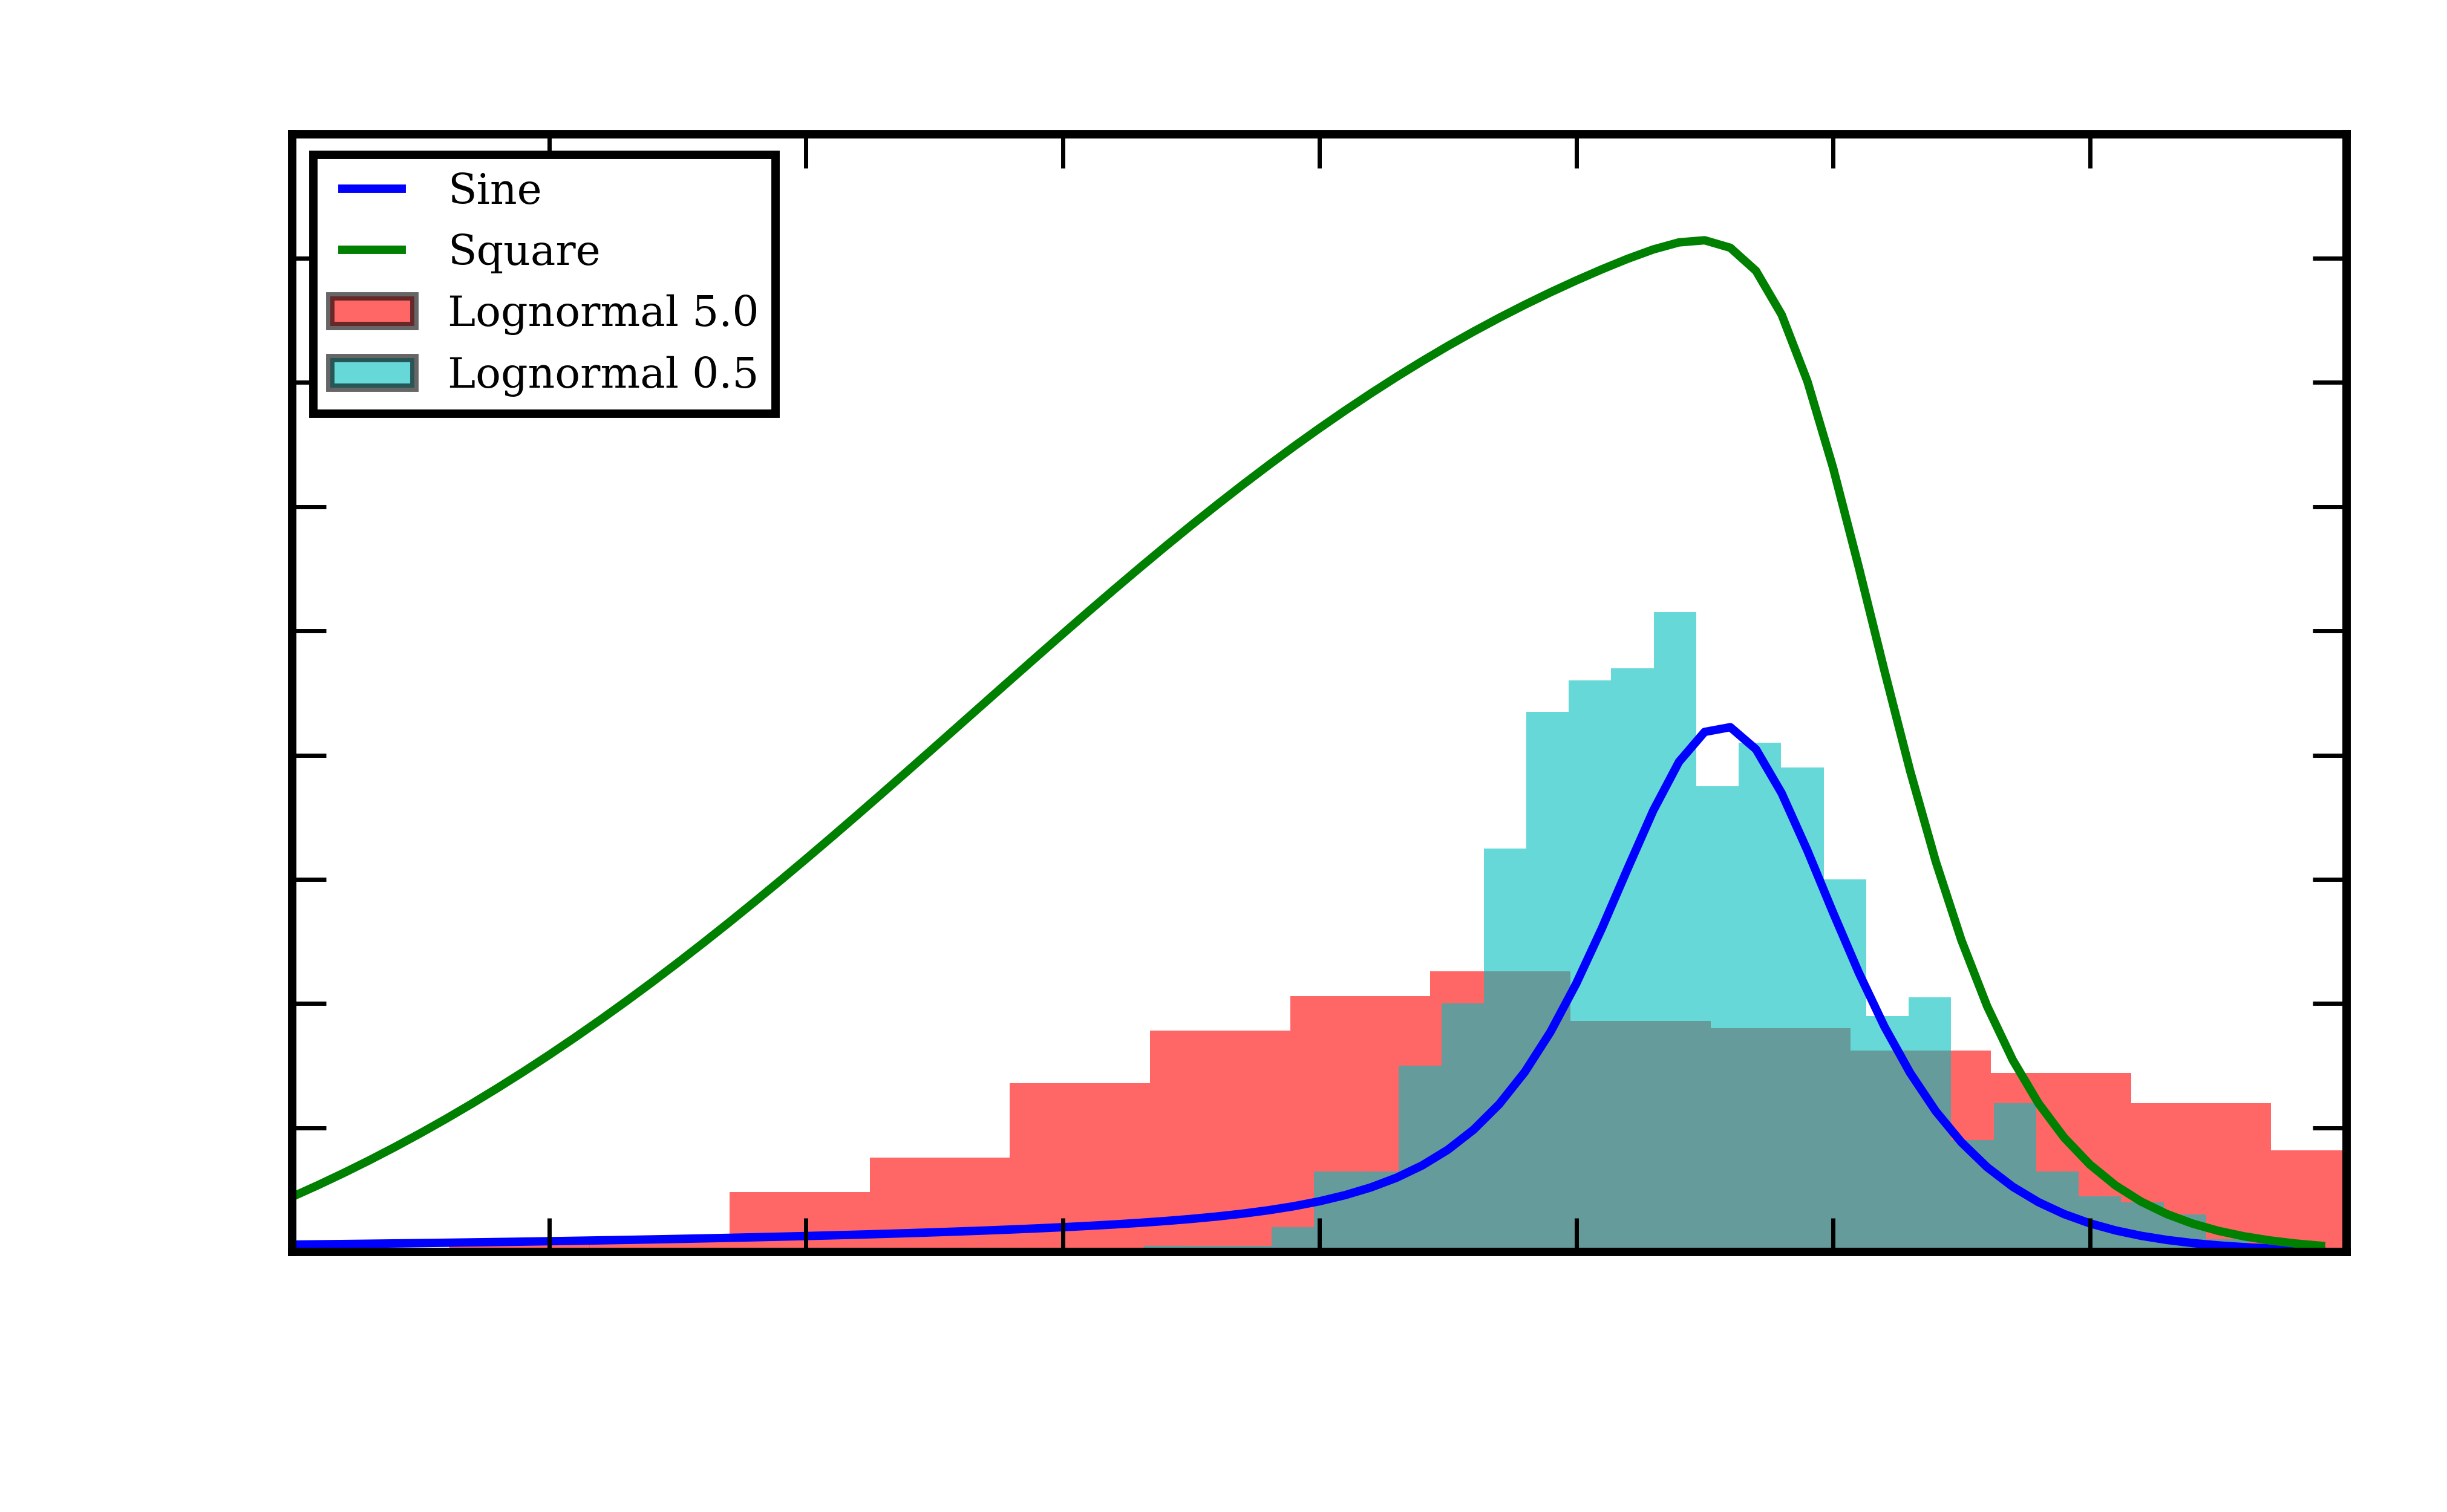
\includegraphics{figures/dist.png}
  \end{center}
\vspace{-3mm}
{\tiny $T=298$K, $K=11$kJ/m$^3$, $h=0.13$, $f=300$kHz, $\alpha=0.1$, $M_s=350$kA/m}
\end{frame}

\begin{frame}
  \frametitle{Applied waveforms of equal power}
  \begin{center}
    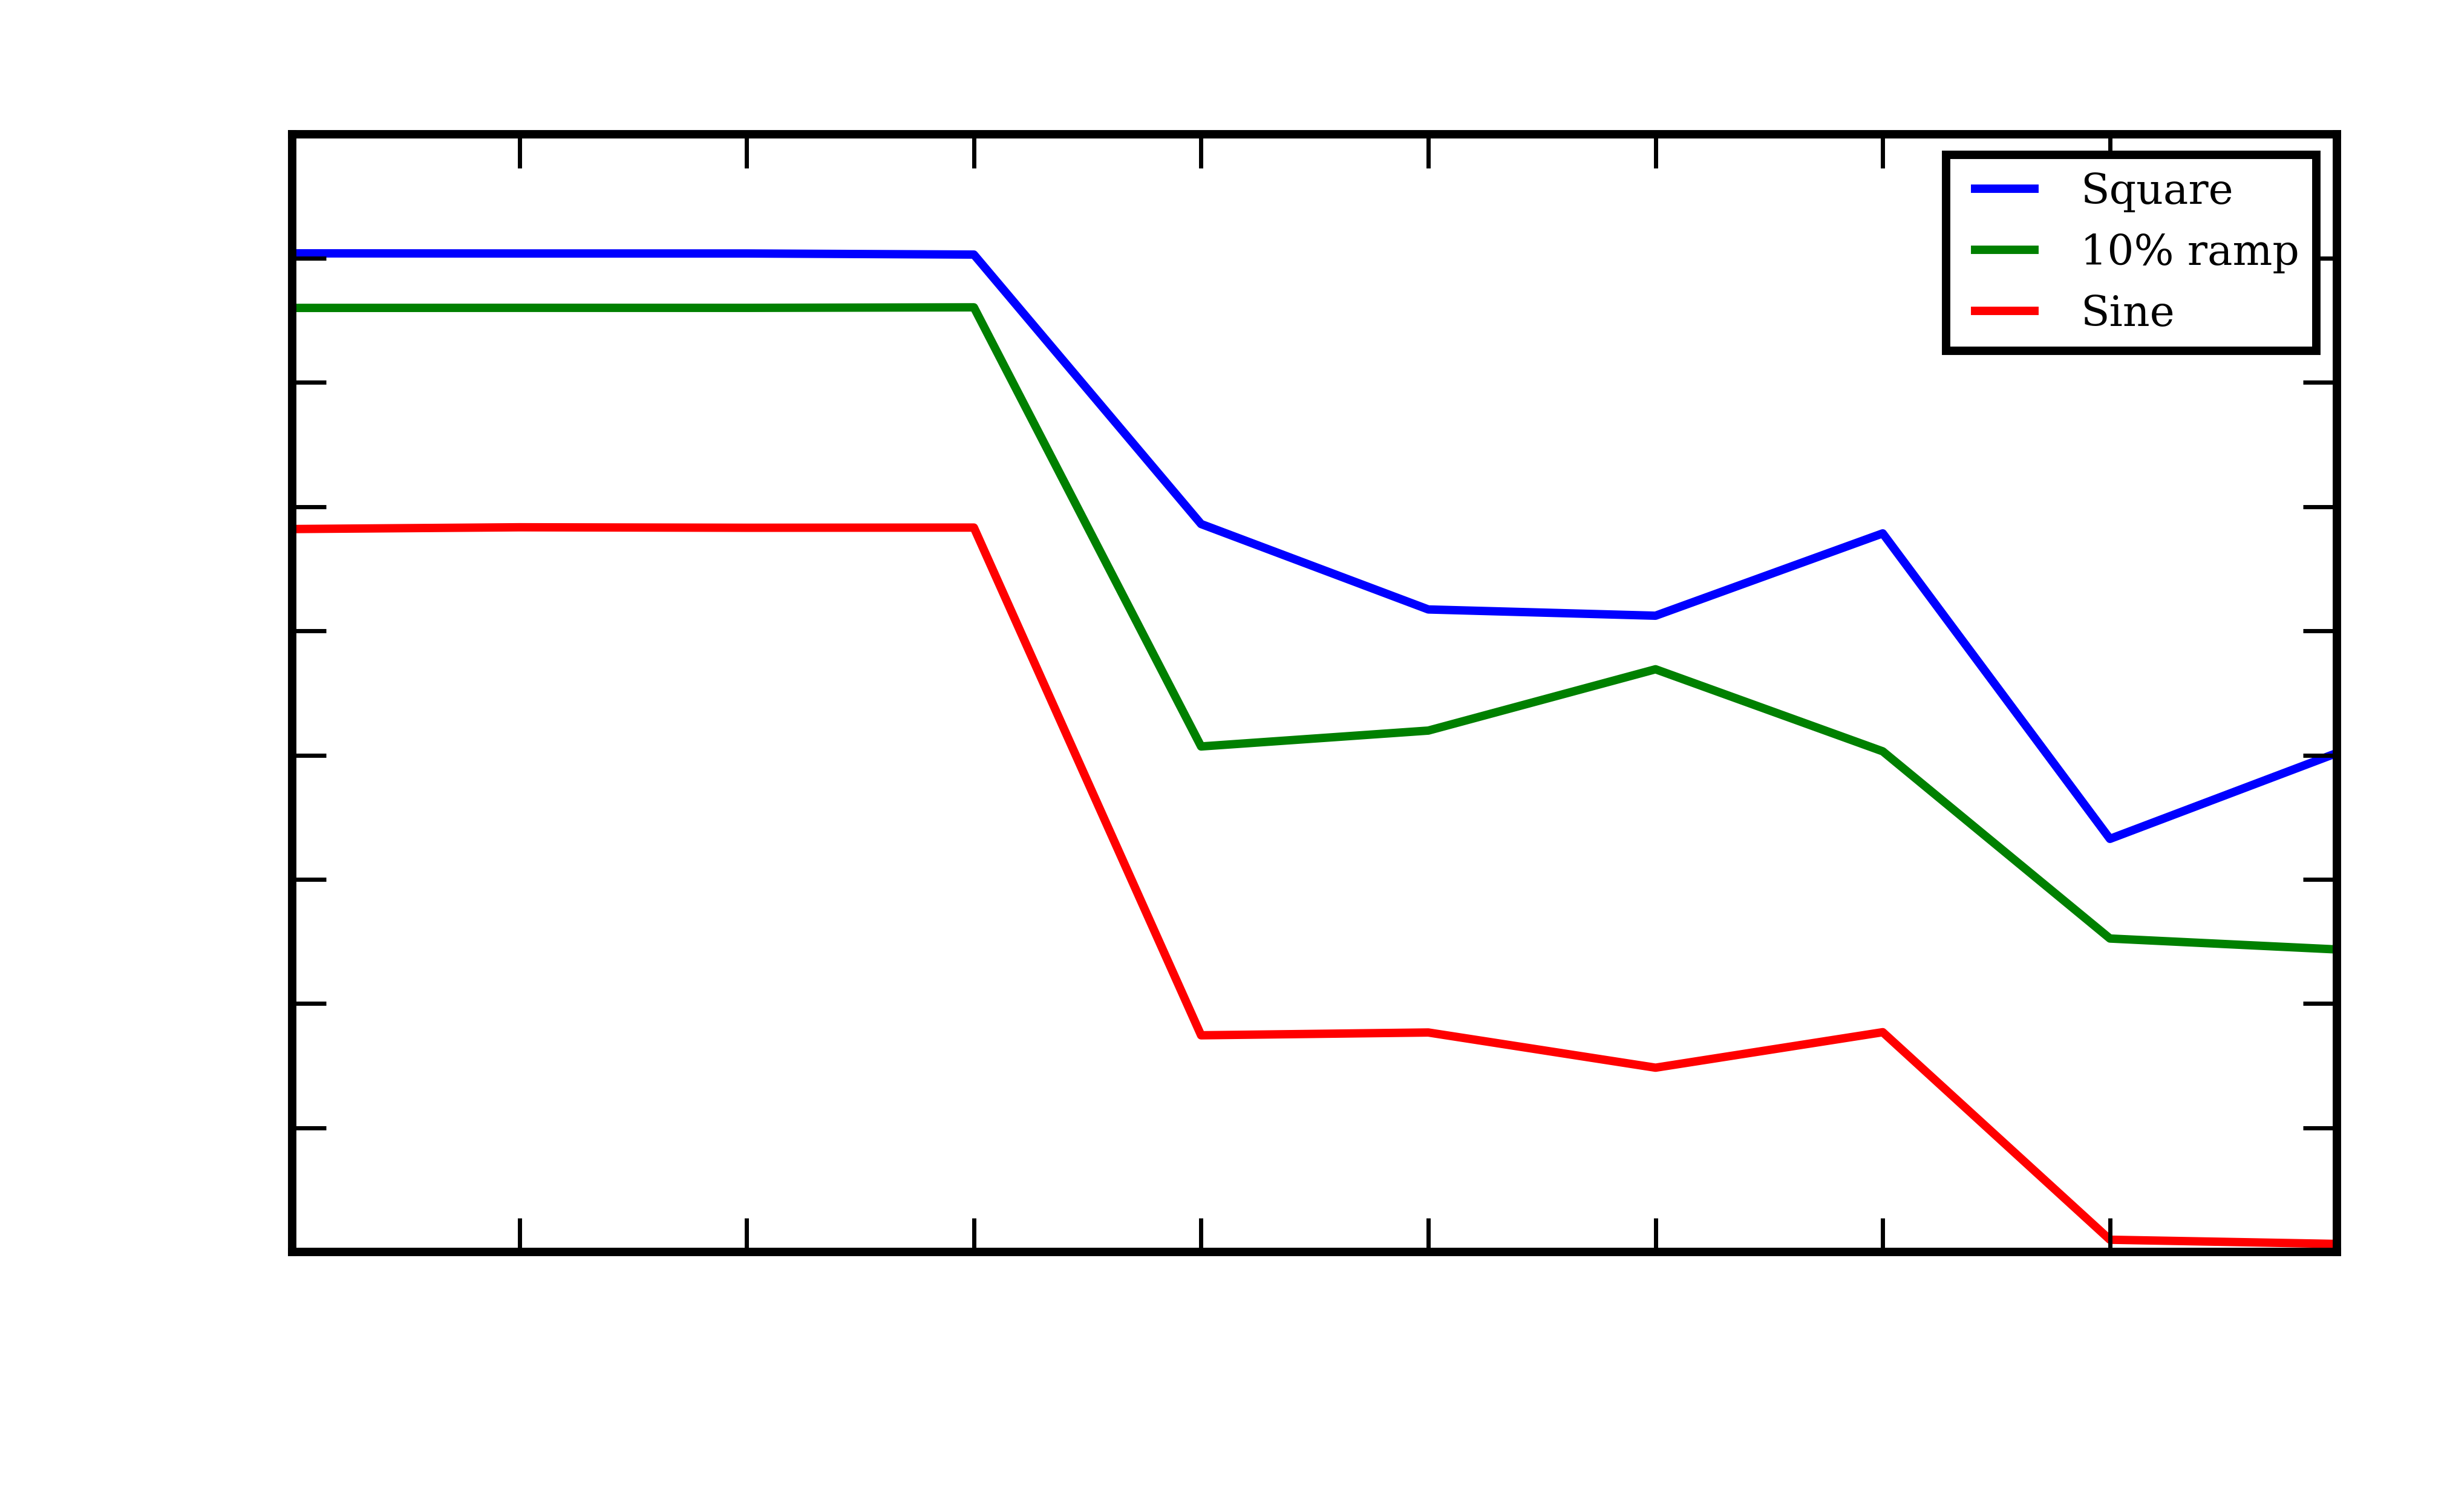
\includegraphics{figures/distsweep.png}
  \end{center}
\vspace{-3mm}
{\tiny $T=298$K, $K=11$kJ/m$^3$, $h=0.13$, $f=300$kHz,
  $\alpha=0.1$, $M_s=350$kA/m, $\bar{r}=9.5$nm}
\end{frame}

\begin{frame}{Conclusions}
  \begin{itemize}
  \item We have introduced an alternative formulation to compute the
    SPL obtained in an applied square wave.
  \item The square waveform can target a large range of particle sizes.
  \item Good SPL can be achieved with broad particle distributions and
    trapezoidal waves.
  \end{itemize}
\end{frame}

\begin{frame}{}
  \begin{center}
      \Large Questions?
  \end{center}
\vspace{7mm}
\begin{center}
  \raisebox{0.3\height}{
\includegraphics[width=0.3\linewidth]{sponsors/icss_square_logo.png}}
  \hspace{6mm}
  
\includegraphics[width=0.3\linewidth]{sponsors/sponsor-wo.eps}

  {
\includegraphics[width=0.3\linewidth]{sponsors/wun.png}}
\end{center}
\end{frame}

\appendix
\end{document}

%%% Local Variables:
%%% mode: latex
%%% TeX-master: t
%%% TeX-engine: xetex
%%% End:
